\documentclass[11pt,a4paper]{article}

\usepackage[T1]{fontenc}
\usepackage[utf8]{inputenc}
\usepackage{mathpazo}
\usepackage[protrusion=true,expansion=false]{microtype}
\usepackage[a4paper,top=25mm,bottom=24mm,left=25mm,right=25mm,headheight=22pt]{geometry}
\usepackage{amsmath,amssymb,mathtools}
\usepackage{graphicx}
\usepackage{xcolor}
\usepackage{booktabs}
\usepackage{tabularx}
\usepackage{longtable}
\usepackage{array}
\usepackage{enumitem}
\usepackage{caption}
\usepackage{placeins}
\usepackage{fancyhdr}
\usepackage{tikz}
\usetikzlibrary{arrows.meta,positioning,calc,fit}
\usepackage{pgfplots}
\pgfplotsset{compat=1.18}
\usepackage[numbers,sort&compress]{natbib}
\usepackage{hyperref}
\usepackage[nameinlink,noabbrev]{cleveref}

\definecolor{Forest}{HTML}{08241F}
\definecolor{DeepForest}{HTML}{021815}
\definecolor{Paper}{HTML}{F6F0E8}
\definecolor{Gold}{HTML}{C8953F}
\definecolor{Rust}{HTML}{8C5138}
\definecolor{Sage}{HTML}{879A8D}
\definecolor{Mist}{HTML}{E7ECE8}
\definecolor{Alert}{HTML}{A63D2F}
\definecolor{Positive}{HTML}{2F6B57}

\hypersetup{
  colorlinks=true,
  linkcolor=Forest,
  citecolor=Rust,
  urlcolor=Rust,
  pdftitle={Financing Cellular-Agriculture Scale-Up under Correlated Technical Risk},
  pdfauthor={Naturalehia},
  pdfsubject={Open financial engineering for cellular agriculture},
  pdfkeywords={cellular agriculture, financial engineering, milestone-contingent claims, portfolio risk, funding liquidity, expected shortfall}
}

\pagestyle{fancy}
\fancyhf{}
\fancyhead[L]{\footnotesize\color{Forest}\textsc{Financing Cellular-Agriculture Scale-Up}}
\fancyhead[R]{\footnotesize\color{Rust}\textsc{Working Paper / Version 2.0}}
\fancyfoot[L]{\footnotesize\color{Sage}Open financial engineering / synthetic study}
\fancyfoot[R]{\footnotesize\color{Forest}\thepage}
\renewcommand{\headrulewidth}{0.4pt}
\renewcommand{\headrule}{\hbox to\headwidth{\color{Gold}\leaders\hrule height \headrulewidth\hfill}}

\setlength{\parindent}{0pt}
\setlength{\parskip}{0.55em}
\setlength{\emergencystretch}{2em}
\setlength{\tabcolsep}{5pt}
\renewcommand{\arraystretch}{1.16}
\setcounter{tocdepth}{1}
\setlist[itemize]{leftmargin=1.45em,itemsep=0.22em,topsep=0.25em}
\setlist[enumerate]{leftmargin=1.65em,itemsep=0.3em,topsep=0.3em}
\captionsetup{font=small,labelfont={bf,color=Forest}}
\renewcommand{\sectionmark}[1]{}
\raggedbottom
\clubpenalty=10000
\widowpenalty=10000
\displaywidowpenalty=10000
\makeatletter
\setlength{\@fptop}{0pt}
\setlength{\@fpsep}{1.25\baselineskip}
\setlength{\@fpbot}{0pt plus 1fil}
\makeatother

\newcommand{\demounit}{\textsc{units per 100}}
\newcommand{\statussynthetic}{\textcolor{Rust}{\textsc{Synthetic}}}
\newcommand{\statusunknown}{\textcolor{Alert}{\textsc{Unknown}}}
\newcommand{\statusimplemented}{\textcolor{Positive}{\textsc{Implemented}}}
\newcommand{\tightnote}[1]{\par\smallskip{\footnotesize\color{Sage}#1}\par}
\newcommand{\result}[1]{\textbf{\color{Forest}#1}}
\newcolumntype{Y}{>{\raggedright\arraybackslash}X}
\newcolumntype{R}{>{\raggedleft\arraybackslash}X}
\newcolumntype{P}[1]{>{\raggedright\arraybackslash}p{#1}}

\newenvironment{paperbox}[1]{%
  \begin{center}\begin{minipage}{0.96\textwidth}%
  \color{Forest}\hrule height 1.2pt\vspace{0.65em}%
  {\large\bfseries #1}\par\smallskip\color{black}%
}{%
  \vspace{0.45em}\color{Gold}\hrule height 0.7pt
  \end{minipage}\end{center}%
}

\begin{document}
\pagenumbering{arabic}
\thispagestyle{empty}
\vspace*{-12mm}
{\small\bfseries\color{Rust}\MakeUppercase{Naturalehia Research \enspace/\enspace Financial Engineering Working Paper}}\par
\vspace{7mm}
{\LARGE\bfseries\color{Forest} Financing Cellular-Agriculture Scale-Up under Correlated Technical Risk}\par
\vspace{2mm}
{\large\color{Forest}Milestone-Contingent Claims, Loss Allocation, and Funding Liquidity}\par
\vspace{5mm}
\color{Gold}\rule{\textwidth}{1.2pt}\color{black}
\vspace{4mm}

\begin{tabularx}{\textwidth}{@{}P{0.20\textwidth}Y@{}}
  \textbf{Author} & Naturalehia Research (collective research authorship)\\
  \textbf{Version} & 2.0 / 1 September 2026\\
  \textbf{Model case} & Ten synthetic project claims; 100 reference principal; 60-month horizon\\
  \textbf{Correspondence} & \href{https://naturalehia.waajacu.com/projects/fostering-cellular-agriculture/}{naturalehia.waajacu.com/projects/fostering-cellular-agriculture}\\
  \textbf{Release status} & Open working paper; not externally peer reviewed\\
\end{tabularx}

\begin{abstract}
Cellular agriculture requires staged capital across research, pilot, demonstration and first-industrial facilities, yet early cash is sparse, technical failures are correlated and repayment rights are often unclear. We ask under what cash rights, loss allocation, funding mechanics, price and external support a correlated milestone portfolio could satisfy investor return and tail-risk constraints without manufacturing value. We define a limited-recourse Multi-Project Milestone Participation and a source-separated, principal-conserving model of project draws, assigned cash, recoveries, unresolved principal and external support. Dependence is represented by complete joint states and a box-and-simplex set of physical probabilities.

In a ten-claim synthetic experiment per 100 of reference principal, the unsupported core has central expected NPV of 0.66 at an assumed 8\% hurdle but a robust adverse expectation of -18.72. Pooling reduces central resolved-loss ES95 by 10.05\%, while the ES99 benefit is zero. A fully funded stack adds 8.98 of central timing drag; a 30\% guarantee transfers external cash but leaves adverse investor inadequacy. A finite 25-candidate participation-by-first-loss screen finds no feasible term, and a subsequent issue-price/support sensitivity finds no funded window at the assumed 8\% hurdle. These are conditional rejection results, not prices or forecasts. Live use requires executed cash rights, empirical joint loss and recovery data, observed investor prices or hurdles, and evidenced provider capacity.
\end{abstract}

\textbf{Keywords:} cellular agriculture; financial engineering; milestone-contingent claims; portfolio dependence; expected shortfall; funding liquidity; partial-credit guarantee.\\
\textbf{JEL classification:} G11, G23, G32, G38, Q14.

\vspace{3mm}
\begin{minipage}{\textwidth}
  \color{DeepForest}\hrule height 0.7pt\vspace{0.55em}
  \footnotesize\textbf{Research-status notice.} This working paper is a synthetic financial-engineering study. It is not an offer, solicitation, investment recommendation, rating, valuation, fairness opinion, or legal, tax, accounting, regulatory or prudential advice. No issuer, security, provider, market price or regulatory treatment has been established. Monetary results are normalized \demounit{} of reference principal.
\end{minipage}
\clearpage

\section{Introduction}

The objective of this research is practical: make it possible for institutional, mission and public capital to finance credible cellular-agriculture work from research into repeatable production without concealing the risk that capital is actually taking. The ethical purpose is to help build an industrial alternative to systems that confine and slaughter animals. That purpose raises the standard of evidence; it does not relax it.

The financing problem is not solved by naming a fund, adding projects, or promising that scale will arrive. Investors need a valuable asset: a defined property right to identifiable cash, a complete account of when capital is at risk, a distribution of loss and return that respects shared shocks, and terms under which the asset can be accepted or rejected. Public and philanthropic institutions need the same visibility from the opposite side: what risk they absorb, when cash can be called, whether support is additional, and whether a private return is being created by productive cash or subsidy.

\begin{paperbox}{Research question}
Under what assigned cash rights, milestone controls, loss allocation, funding mechanics, issue price and external support can a correlated portfolio of cellular-agriculture projects satisfy an investor's return and tail-risk constraints without counting promises as cash or relabeling transfers as project value?
\end{paperbox}

Biomedical research-backed obligation proposals established an important intellectual precedent by combining uncertain development programs, staged asset value and structured claims \citep{fernandez2012rbo,fagnan2013cancer,fagnan2014orphan}. The present design borrows the discipline of pooling, cash waterfalls and explicit guarantees, but it does not assume that cellular-agriculture projects possess comparable licensing markets, development probabilities, or debt capacity. It begins one level lower: every project must first connect to a common financial interface, and every unit of investor return must trace to an enforceable source.

This paper makes six contributions:

\begin{enumerate}
  \item It defines the economic asset before the legal wrapper: a limited-recourse participation in dated, source-budgeted project cash, recovery and continuing exposure.
  \item It gives one core construction and two alternative risk-allocation variants without claiming that tranching or guarantees create underlying project value, and supplies an explicit asset-to-liability bridge for non-par claims.
  \item It formulates cash conservation, expected shortfall, physical-probability ambiguity and the finite investor-mandate screen as explicit mathematical programs with retained adverse witnesses.
  \item It separates project return, liability cash shortfall, provider transfer and funding liquidity so that one balance sheet cannot be counted twice.
  \item It turns non-investability into a useful output by stating measurable rejection conditions and the evidence needed for a live issuance.
  \item It separates verified mechanics from empirical underwriting and defines the controlled cohort and transaction evidence needed before synthetic risk can become an investable estimate.
\end{enumerate}

\begin{paperbox}{Key finding: the current terms are defined but not shown financeable}
The synthetic core is barely positive at the central probability mix, yet its robust adverse expected NPV is -18.72. Central ES95 diversification exists but disappears at ES99. A funded junior layer introduces 8.98 of central prefunding drag, and a 30\% guarantee improves investor NPV only by adding external provider cash; it still leaves a large adverse gap and an unfunded provider budget requirement. The finite screen rejects all 25 declared same-pool \((q,A)\) candidates under an illustrative risk budget. This is evidence that the method can expose a financing gap, not evidence about any live company or untested term.
\end{paperbox}

\section{The financing problem}

\subsection{Why research-to-industry scale-up resists ordinary debt}

Cellular-agriculture projects cross qualitatively different stages. Shared science and platform research can create broad public and private option value while producing no near-term debt-service cash. Pilot and demonstration assets may generate operational evidence but remain exposed to biology, contamination, media supply, equipment integration, product qualification and buyer acceptance. First-industrial facilities add construction, commissioning, throughput, yield, cost and market risks at larger capital scale. Published techno-economic work illustrates why scale, media, mass transfer and process assumptions remain economically decisive, while reviews show that materially different assumptions still drive modeled outcomes \citep{humbird2021scale,pasitka2024continuous,goodwin2024scoping}. Food-safety hazards and regulatory controls create another distinct evidence path \citep{fao2023safety}. Repeat facilities can become more debt-like only after these risks are evidenced and contractual revenues exist.

An ordinary fixed-rate loan presumes a sufficiently stable repayment source. A conventional venture investment can absorb more uncertainty but may be unsuitable for institutions seeking dated cash and bounded exposure. A single project can be too concentrated for either. The engineering task is therefore not to disguise early uncertainty as credit. It is to create a transparent progression of claims whose cash rights, loss states and evidence requirements mature with the underlying work. Dynamic-leverage research in biomedicine supports this sequencing: equity-like risk absorbs early discovery uncertainty and debt is introduced only as risk becomes measurable \citep{montazerhodjat2016dynamic}.

\subsection{The five separations that prevent false value}

The proposed standard maintains five separations throughout:

\begin{enumerate}
  \item \textbf{Investor cash versus contractual principal.} Cash paid is a dated flow; principal is a contractual balance. At-par draws may make them numerically equal, but they are not conceptually interchangeable.
  \item \textbf{Project cash versus external support.} Commercial, licensing, royalty and recovery receipts are produced by project rights. Guarantee payments are transfers from another balance sheet.
  \item \textbf{Resolved loss versus continuing exposure.} A delayed or unresolved claim is not cash and is not automatically a realized loss.
  \item \textbf{Expected loss versus price, provision and capital.} A provider's expected claim cost is not, by itself, a market premium, IFRS~9 expected-credit-loss allowance, IFRS~13 fair value, fiscal subsidy estimate or regulatory capital number \citep{ifrs9,ifrs13,omb2025a11,eu2024financialregulation,basel2026framework}.
  \item \textbf{Mission impact versus financial return.} Animal displacement and welfare benefit require their own causal evidence. They do not substitute for investor cash flow.
\end{enumerate}

These are not merely disclosure preferences. They are conservation boundaries. If a proposed return cannot be located on one side of a real contract, it is not part of the asset.

\section{Related financial engineering and design departure}

\subsection{Research-backed obligations and correlation}

Fernandez, Stein and Lo propose pooling biomedical-development assets in a bankruptcy-remote vehicle financed by senior debt, junior debt and equity, with repayment materially dependent on sale or licensing of development rights \citep{fernandez2012rbo}. Later work applies the idea to smaller orphan-disease portfolios \citep{fagnan2014orphan}. The relevance here is not either simulated return level. It is the architectural idea that heterogeneous research risks can be represented as assets only when the vehicle controls transferable value and the portfolio, waterfall, triggers and liquidity are modeled together.

Portfolio size alone is not diversification. Work on financing low-probability ``long shots'' emphasizes that even modest common dependence can undermine apparently safe senior claims and that tranching cannot convert a negative-NPV pool into a positive-NPV pool \citep{hull2019longshots}. Correlated-development analysis reaches the same caution through explicit common-factor models \citep{lo2021correlated}. Structured claims whose losses concentrate in bad aggregate states can resemble economic catastrophe bonds even when their unconditional expected loss appears modest \citep{coval2009catastrophe}. Cellular agriculture has obvious common factors: related cell platforms, shared media and growth-factor suppliers, similar scale-up physics, common equipment vendors, regulatory pathways, buyers and follow-on capital markets. The present model therefore starts from complete joint states. It never obtains a portfolio default distribution by multiplying marginal defaults as if independent.

\subsection{Risk measures, ambiguity and funding liquidity}

Expected shortfall is used because it is a coherent, subadditive tail measure and can be evaluated directly on a finite scenario distribution \citep{artzner1999coherent,rockafellar2000cvar}. Parameter uncertainty is not hidden inside a single precise expected return: the model evaluates each primary metric over a disclosed set of physical probability measures, following the multiple-prior discipline that an investor's conclusion should remain visible under plausible parameter variation \citep{garlappi2007multiprior}. This is robust sensitivity analysis, not distributional calibration.

Funding timing is a separate source of risk. In private markets, subscription credit lines bridge capital calls against committed but undisbursed investor capital \citep{bis2021privatemarkets}. ILPA recommends disclosure of facility size and balance, draw duration, rates, fees, purpose and returns both with and without a subscription facility \citep{ilpa2020subscription}. The Basel liquidity framework likewise distinguishes a future funding commitment from cash already held and prohibits double counting the same liquidity item \citep{basel2019lcr40}. Those references motivate the paper's cash-only discipline; they do not establish that ILPA guidance or Basel rules govern a future cellular-agriculture vehicle.

\subsection{Guarantees and realized blended-finance analogues}

The biomedical megafund guarantee literature shows why mean expected claims are an incomplete measure of the guarantor's commitment: adverse cash calls can be large even when mean cost appears modest \citep{fagnan2013cancer}. The Global Health Investment Fund provides a realized analogue of a mission-oriented pool using milestone and royalty instruments with partial downside protection from philanthropic/public guarantors. Its reported mechanism absorbed the first 20\% of losses and shared subsequent losses, leaving private investors exposed \citep{worldbank2017ghif}. This supports the legitimacy of transparent partial loss sharing; it does not validate cellular-agriculture probabilities, recoveries or investor demand.

Blended-finance discipline requires a development rationale, additionality, minimum concessionality, commercial sustainability and transparency about the support used to mobilize private capital \citep{ifcblended}. Accordingly, any first-loss or guarantee value in this paper is shown separately from project economics.

\subsection{A documented public-credit precedent in cellular agriculture}

Meatable announced in September 2024 that it had been awarded a EUR 7.6 million Innovation Credit from the Netherlands Enterprise Agency to improve cultivated-meat productivity and reduce costs before commercialization \citep{meatable2024credit}. This is issuer-reported evidence of a named public development-credit award in cellular agriculture; it is not evidence of the exact legal recipient, individualized decision, cash receipt, draw schedule, probability of technical success, repayment cash, loss, or private-market value.

The official 2024 programme opening set a 3\% annual base rate and a 15\% fixed premium for technical-development projects \citep{nl2024innovationcredit}. Generic programme documents describe project reporting and cash-flow forecasts, include a template for a first-ranking pledge over identified project assets, and state that the credit, accrued interest and fixed premium are repayable unless relief is granted \citep{rvo2024obligations}. Current programme guidance, which postdates the announced award, describes relief after technical failure or loss of market prospects as a case-specific request that the agency may accept in whole or in part, not an automatic payoff formula or an award-specific term \citep{rvo2026following}.

The precedent matters because it shows a candidate public-credit architecture for development risk rather than treating early research as ordinary bank debt. It also exposes the data a private pool would still need: the individualized award decision, borrower, approved budget, advances, milestone tests, exact repayment schedule, pledged assets, other financing, amendments, remission decision and actual settlement. The public record therefore supports mechanism research while remaining ineligible as a price, expected-return observation or calibrated loss history.

The adverse company outcome is now public too. On 19 December 2025 Agronomics reported that Meatable's board and shareholders had resolved to dissolve Meatable B.V. and related group companies, terminate operating activities and conduct an orderly wind-down after the company was unable to obtain continued funding; Agronomics also reported writing its own Meatable investment from a carrying value of GBP 11.9 million to zero \citep{agronomics2025meatabledissolution}. This is evidence of a company wind-down decision and an equity-investor write-off, not evidence that the Innovation Credit defaulted, was accelerated or remitted, or produced any creditor recovery. The legal dissolution date, RVO claim status, outstanding public-credit principal, security enforcement and liquidation proceeds remain unidentified.

\subsection{Where this proposal differs}

The design does not begin with leverage or a rated senior tranche. It begins with a standardized claim ledger. It does not count company valuations, generic intellectual property, unused payer capacity or refinancing proceeds as operating cash. It does not assume a liquid secondary market for failed or partially developed assets. It does not force one instrument across all stages. Finally, its central result is allowed to be rejection.

\section{Definition of the underlying asset}

\subsection{The project financial interface}

Each candidate project is normalized through the same interface \citep{fca2026interface}. For project \(i\), the interface must identify the items in \cref{tab:interface} before inclusion.

\begin{table}[htbp]
\centering
\caption{Minimum project financial interface}
\label{tab:interface}
\begin{tabularx}{\textwidth}{@{}P{0.19\textwidth}Y Y@{}}
\toprule
\textbf{Component} & \textbf{Required representation} & \textbf{Reason for investors} \\
\midrule
Capital & Dated commitment, draw, fee and milestone schedule & Determines cash paid, liquidity need and the value of stopping later draws \\
State & Observable milestone, delay, stop, conversion and resolution states & Prevents narrative progress from replacing contractual conditions \\
Principal & Creation, repayment, conversion, write-off and continuing balance & Separates exposure from cash and realized loss \\
Success cash & Named commercial, licensing, royalty, capacity, offtake or exit right, with source budget & Establishes where non-principal return can legally come from \\
Recovery & Priority, amount, timing and evidentiary status & Determines loss-given-resolution without assuming salvage \\
Shared risk & Biology, scale-up, supplier, regulatory and buyer factor exposure & Makes dependence and concentration explicit \\
Evidence & Contractual, observed, estimated, synthetic or unknown status & Prevents unknown values from entering as zero \\
\bottomrule
\end{tabularx}
\end{table}

The investor owns a pro-rata, limited-recourse right to the admitted project claims, specifically assigned success cash, identified recoveries and any separately documented support. The investor does not automatically own a facility, company equity, company value, speculative intellectual property, a public sponsor's unused balance sheet, or a manager's promise.

\subsection{Admission is a falsifiable contract test}

A project is admitted only if the claim is unique, cash-source budgets do not overlap, milestone evidence can control draws, principal identities reconcile, the common calendar is explicit, and all material factor exposures are declared. Admission verifies representability; it does not validate the project or imply financeability. Missing evidence remains \statusunknown{}, never zero.

For a live pool, claim data must be authenticated against executed contracts, controlled data-room records, verifier certificates and settlement instructions. At minimum, legal diligence must establish transferability, perfection, priority, limited recourse, insolvency treatment and enforceability in each relevant jurisdiction.

\section{The candidate instrument}

\subsection{Core: Multi-Project Milestone Participation}

The core is one disclosed claim across a fixed set of project claims. Investors make callable commitments. Each project can draw only at dated milestones. Failure or non-achievement can stop later funding. Actual project receipts and recoveries pass through pro rata after explicit pool cost. The claim is not promised a fixed coupon independent of project cash; return arises only from identified rights.

\begin{figure}[htbp]
\centering
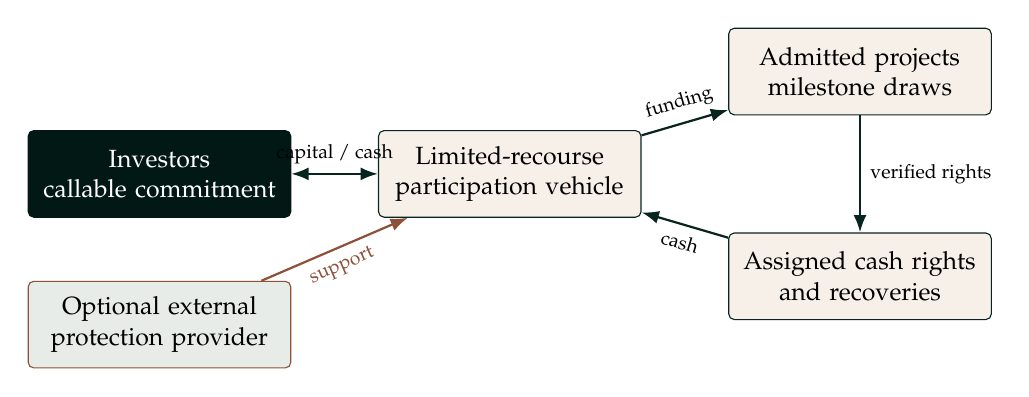
\begin{tikzpicture}[
  node distance=8mm and 11mm,
  box/.style={draw=Forest,rounded corners=2pt,fill=Paper,minimum height=11mm,text width=31mm,align=center,font=\small},
  dark/.style={box,fill=DeepForest,text=white,draw=DeepForest},
  support/.style={box,fill=Mist,draw=Rust},
  arrow/.style={-{Latex[length=2.2mm]},thick,draw=Forest},
  both/.style={{Latex[length=2.2mm]}-{Latex[length=2.2mm]},thick,draw=Forest}
]
\node[dark] (investors) {Investors\\callable commitment};
\node[box,right=of investors] (vehicle) {Limited-recourse\\participation vehicle};
\node[box,right=of vehicle,yshift=13mm] (projects) {Admitted projects\\milestone draws};
\node[box,right=of vehicle,yshift=-13mm] (rights) {Assigned cash rights\\and recoveries};
\node[support,below=of investors] (provider) {Optional external\\protection provider};
\draw[both] (investors) -- node[above,font=\scriptsize]{capital / cash} (vehicle);
\draw[arrow] (vehicle) -- node[above,sloped,font=\scriptsize]{funding} (projects);
\draw[arrow] (projects) -- node[right,font=\scriptsize]{verified rights} (rights);
\draw[arrow] (rights) -- node[below,sloped,font=\scriptsize]{cash} (vehicle);
\draw[arrow,draw=Rust] (provider) -- node[below,sloped,font=\scriptsize,text=Rust]{support} (vehicle);
\end{tikzpicture}
\caption{Economic architecture. Project cash and external support remain visibly separate.}
\label{fig:architecture}
\end{figure}

\subsection{Variant 1: fully funded first-loss and priority claims}

Investors subscribe a reserve at inception. A funded first-loss claim occupies horizon principal-cash-shortfall coordinates beginning at zero; priority claims attach above it. Contractual-principal cash and unused reserve pay principal most senior first. Assigned non-principal cash pays priority up to a lifetime cap and then flows to the first-loss residual. Buyer direct costs and pool costs are separate pro-rata calls rather than tranche principal. Returned reserve is capital, not profit.

The asset-to-liability bridge does not assume that cash paid for an asset, contractual asset principal and issued principal are equal. Let \(A_{is}\) be project \(i\)'s acquisition and primary-funding use in state \(s\), excluding buyer direct cost. The funded limit is set project by project:
\begin{align}
R_i&=\max_{s\in\mathcal S}A_{is}, & R&=\sum_i R_i,\\
A_s&=\sum_i A_{is}, & U_s&=R-A_s,
\end{align}
where \(R\) is both reserve subscription and issued tranche principal, and \(U_s\) is unused reserve returned at the horizon. This deliberately uses the sum of project maxima, not the maximum aggregate use in one state; projects can require liquidity in different states.

Let \(P_s\) be contractual-principal cash received by the analysis horizon. The liability ledger is
\begin{align}
D_s&=\min\bigl(R,P_s+U_s\bigr),\\
Q_s&=R-D_s,\\
S_s&=\max\bigl(0,P_s+U_s-R\bigr),
\end{align}
where \(D_s\) is principal cash distributable to issued claims, \(Q_s\) is their horizon principal-cash shortfall after the single aggregate canonicalization described below, and \(S_s\) is cash above unpaid issued principal that enters the declared non-principal waterfall. For a tranche with attachment \(a_j\) and detachment \(d_j\),
\begin{equation}
Q_{js}=\min\!\left(\max(Q_s-a_j,0),d_j-a_j\right).
\label{eq:tranche-shortfall}
\end{equation}
Thus a 0--20 first-loss claim absorbs the first 20 of \(Q_s\), while an attaching priority claim receives principal cash first.

Before tranche layering, the engine canonicalizes aggregate \(Q_s\) once: a non-negative residual no greater than \(\tau(R)=10^{-9}+16\varepsilon_{\mathrm{double}}\max(1,|R|)\) is set to zero. No tranche applies an independent tolerance. The resulting once-canonicalized \(Q_s\) is the liability observable used throughout the funded stack.

The asset ledger remains separate:
\begin{equation}
L_s=\sum_i\ell_{is},\qquad O_s=\sum_i u_{is}.
\end{equation}
Here \(L_s\) is contractual principal written off on resolved paths and \(O_s\) is contractual principal still outstanding on continuing paths. The model asserts no causal allocation, impairment identity or post-horizon recovery value linking \(L_s\), \(O_s\) and \(Q_s\). Pooled cash identifies the liability shortfall but not which asset economically caused it. Aggregate contractual-principal limit less \(A_s\) is reported only as a principal-limit capacity diagnostic: the limit need not equal principal created or acquired in that state, so the difference is not a price, discount, premium or fair value.

\begin{table}[htbp]
\centering
\caption{Non-par hand checks for the exact asset-to-liability bridge}
\label{tab:bridge-hand-checks}
\small
\begin{tabularx}{\textwidth}{@{}YrrrrrrY@{}}
\toprule
\textbf{State} & \(R=A_s\) & \textbf{Principal limit} & \(P_s\) & \(L_s\) & \(O_s\) & \(Q_s\) & \textbf{Conclusion} \\
\midrule
Resolved 8-for-10 & 8 & 10 & 8 & 2 & 0 & 0 & Asset loss; no liability cash shortfall \\
Performing 12-for-10 & 12 & 10 & 10 & 0 & 0 & 2 & Liability cash shortfall; no asset loss \\
Continuing 8-for-10 & 8 & 10 & 3 & 0 & 7 & 5 & Outstanding asset and cash shortfall remain distinct \\
\bottomrule
\end{tabularx}
\tightnote{All amounts are synthetic \demounit{}. These rows demonstrate accounting mechanics, not market price, impairment, recovery or investability.}
\end{table}

When contractual-principal cash and reserve return arrive in the same month, they have equal seniority. For a simultaneous surplus \(S_{s,t}\), the engine records the source memo pro rata,
\begin{equation}
S^P_{s,t}=S_{s,t}\frac{P_{s,t}}{P_{s,t}+U_{s,t}},\qquad
S^U_{s,t}=S_{s,t}-S^P_{s,t},
\end{equation}
and uses the same ratio for the paid-principal source memo. This is a deterministic convention for fungible cash, not observed provenance; both sources enter one waterfall, so the split changes neither total cash nor tranche entitlement.

This variant changes payment timing and priority. It does not change project receipts, contractual writeoff, continuing principal, common-factor dependence or diversification. Full prefunding can reduce call risk but introduces negative carry when capital waits in reserve. The ten-claim illustration below remains the documented at-par draw-equals-principal baseline; the explicit bridge above controls any non-par claim. No cross-version equivalence inference is made from that baseline.

\subsection{Funding-liquidity extension: design and publication boundary}

Full prefunding is a conservative boundary, not the only possible funding method. A callable-capital and warehouse design could reduce idle-cash drag only by replacing it with explicitly measured call-timing, provider-credit, collateral, maturity and refinancing risk. Let \(J\) be funded subordinated cash present at close, \(C_{s,t}\) settled capital-call cash, \(W^+_{s,t}\) settled warehouse advances, \(W_{s,t}\) warehouse principal, \(E_{s,t}^{\mathrm{pf}}\) pro-forma eligible funded cost, \(K_{s,t}\) independently declared eligible collateral, \(H\) the facility limit and \(\alpha\) the contractual advance rate. A candidate borrowing-base control is
\begin{equation}
BB_{s,t}=\min\!\left\{H,\alpha K_{s,t},\max\!\left(0,E_{s,t}^{\mathrm{pf}}-J_{s,t}^{\mathrm{available}}\right)\right\},
\qquad W_{s,t}\leq BB_{s,t}.
\label{eq:warehouse-bb}
\end{equation}
The last term prevents the same funded junior cash from being represented again as warehouse-funded basis. Neither undrawn commitment nor unused facility limit is cash or loss absorption.

An implementable funding policy must be nonanticipative: calls and advances at month \(t\) are functions \(\pi_t(\mathcal F_t)\) only of information then observed. Two paths with the same history through \(t\) must therefore produce the same action. Acquisition and primary-funding uses are tested before same-month project receipts; settled calls first cure due warehouse principal, and project receipts then sweep warehouse debt according to the fixed priority. Interest, fees, buyer-direct cost and pool cost require separate cash and cannot expand the eligible borrowing base.

Any positive funding shortfall, protection deficit, facility breach or unpaid maturity invalidates the supplied successful project path from that month onward. Investor NPV is then unavailable rather than calculated from cash that depended on the missed funding. A complete extension must also distinguish terminal exposure from realized provider loss, model recovery rather than infer it, preserve provider identity and concentration, and charge for callable capacity as well as drawn debt.

This paper does not report a quantitative warehouse or callable-capital result. The funding-liquidity extension remains a proposed research design until those controls, a nonanticipative policy and a complete ten-claim performance fixture pass independent review. Accordingly, the 8.98 central prefunding drag reported below is a baseline cost to investigate, not a saving claimed to be available.

\subsection{Variant 2: failure-contingent partial-credit guarantee}

The alternative guarantee attaches only to the untranched multi-project participation core defined in Section~5.1. Let \(g\) be the covered share, \(\Gamma\) the provider's legal cash cap and \(L_s\) final resolved loss. With full provider performance,
\begin{align}
G_s &= \min(gL_s,\Gamma),\\
L^{\mathrm{retained}}_s &= L_s-G_s.
\end{align}
The ten-claim experiment uses \(g=30\%\), \(\Gamma=30\), and month-60 settlement. Continuing exposure is not covered. The guarantee creates an external claim on a provider and a corresponding contingent liability for that provider; it does not create project revenue or diversification.

The funded stack and guarantee are intentionally alternative constructions. Combining them would require a new attachment, recovery, subrogation and no-double-recovery waterfall.

\section{Formal model}

\subsection{Timeline and information set}

The analysis date is month zero and the contractual horizon is month \(T\). At the beginning of month \(t\), the vehicle observes the history \(\mathcal F_t\), verifies any milestone and determines the draw permitted by the contract. Investor contributions and other settled funding arrive before acquisition, primary-funding and pool-cost uses. Project receipts and recoveries dated in month \(t\) arrive only after those uses and then enter the applicable waterfall. This ordering prevents a same-month success receipt from curing a funding gap that occurred before the receipt. Any dynamic call, draw or funding policy must be \(\mathcal F_t\)-measurable; the retained experiment evaluates fixed complete paths and does not infer a live policy from future outcomes.

\subsection{Indexing, flows and balances}

Projects are indexed by \(i\in\{1,\ldots,n\}\), complete joint states by \(s\in\mathcal S\), and months by \(t\in\mathcal T\). Define:

\begin{itemize}
  \item \(d_{ist}\): investor-funded project draw;
  \item \(c_{ist}\): explicit pool cost attributable to the state;
  \item \(r^{P}_{ist}\): contractual-principal cash returned;
  \item \(x_{ist}\): assigned non-principal success cash;
  \item \(\rho_{ist}\): cash recovery after failure or resolution;
  \item \(u_{is}\): continuing contractual principal at the horizon;
  \item \(\ell_{is}\): resolved contractual-principal loss;
  \item \(e_{is}\): evidenced conversion or other non-cash extinguishment.
\end{itemize}

For state \(s\), the unsupported investor net cash at month \(t\) is
\begin{equation}
CF_s(t)=-\sum_i d_{ist}-c_{st}+\sum_i\bigl(r^{P}_{ist}+x_{ist}+\rho_{ist}\bigr).
\label{eq:cashflow}
\end{equation}
The cash-source identity is checked independently so that commercial, licensing/royalty, recovery and external-support sources equal the receipts assigned to the claim, without double counting principal classification.

For each claim and path, contractual principal must conserve:
\begin{equation}
b^{\mathrm{open}}_{is}+b^{\mathrm{created}}_{is}
=r^{P}_{is}+e_{is}+u_{is}+\ell_{is}.
\label{eq:principal}
\end{equation}
Continuing principal \(u_{is}\) is exposure: it is neither a horizon cash receipt nor a resolved loss. A payment in kind is not cash. Refinancing proceeds are liquidity unless they extinguish the investor's claim with real cash.

For the funded stack, let \(R\) be total issued principal and reserve subscription, \(Z_s=P_s+U_s\) the contractual-principal cash plus unused reserve available to issued claims, and \(K_j=d_j-a_j\) tranche \(j\)'s notional. Then
\begin{align}
D_s&=\min(R,Z_s), & Q_s&=R-D_s,\\
Q_{js}&=\min\!\bigl(\max(Q_s-a_j,0),K_j\bigr),
&D_{js}&=K_j-Q_{js}.
\label{eq:funded-payoff}
\end{align}
If \(S_s=\max(0,Z_s-R)\) is cash above unpaid issued principal and \(B\) is the priority claim's lifetime non-principal cap, aggregate non-principal allocations are
\begin{equation}
X_s^{M}=\min(B,S_s),\qquad X_s^{J}=S_s-X_s^{M}.
\label{eq:nonprincipal-payoff}
\end{equation}
The implementation applies the same priorities recursively by month to preserve payment timing and WAL. Equations~\eqref{eq:funded-payoff}--\eqref{eq:nonprincipal-payoff} show that tranche claims exhaust, but cannot exceed, the fixed pool cash.

\subsection{Investor return}

At annual-effective hurdle \(h\), state NPV is
\begin{equation}
V_s(h)=\sum_{t\in\mathcal T}\frac{CF_s(t)}{(1+h)^{t/12}}.
\label{eq:npv}
\end{equation}
For probability vector \(p\), expected NPV is \(\mathbb E_p[V(h)]=\sum_s p_sV_s(h)\). The hurdle is an investor decision input, not a probability and not a model-produced fair discount rate. The experiment uses 8\% for the core/common comparison, 15\% for the funded first-loss class, and 8\% for the funded priority class. These values are synthetic and not evidence of market demand.

\subsection{Physical probability ambiguity}

Instead of declaring one calibrated distribution, the model defines an admissible set
\begin{equation}
\mathcal P=\left\{p:\ \underline p_s\le p_s\le\overline p_s,\ \sum_{s\in\mathcal S}p_s=1\right\},
\label{eq:polytope}
\end{equation}
with optional event and marginal constraints in the extended engine. These are candidate \emph{physical} probability measures. They are not risk-neutral probabilities, market-implied prices, posterior confidence intervals or regulatory scenarios.

For any metric linear in probabilities, robust endpoints are exact linear programs:
\begin{equation}
\underline M=\min_{p\in\mathcal P}\sum_s p_sM_s,
\qquad
\overline M=\max_{p\in\mathcal P}\sum_s p_sM_s.
\end{equation}
Each endpoint can have a different witness \(p\). Minimum and maximum rows in a table therefore cannot be assembled into a single composite scenario.

\subsection{Loss tails and diversification}

Let \(L_s=\sum_i\ell_{is}\). For a finite loss variable \(Z_s\), confidence level \(\alpha\) and physical measure \(p\), expected shortfall is
\begin{equation}
\operatorname{ES}^{p}_{\alpha}(Z)
=\min_{\eta\in\mathbb R}\left\{\eta+\frac{1}{1-\alpha}
\sum_s p_s\max(Z_s-\eta,0)\right\}.
\label{eq:es}
\end{equation}
This is the probability-weighted mean loss in the worst \(1-\alpha\) tail, with fractional boundary-state allocation when required \citep{rockafellar2000cvar}. The engine evaluates the same operator on NPV shortfall \(\max(-V_s,0)\) and optimizes each reported tail endpoint over \(p\in\mathcal P\). Each endpoint retains its own complete probability and fractional-tail witness.

The reported diversification benefit compares pooled loss ES with the sum of standalone-claim loss ES under the same declared probability measure:
\begin{equation}
D_{\alpha}=\sum_i \operatorname{ES}_{\alpha}(\ell_i)-\operatorname{ES}_{\alpha}(L).
\end{equation}
A positive \(D_{\alpha}\) is a measured distributional effect, not newly created cash. If \(D_{0.99}=0\), the severe common tail has defeated the measured pooling benefit at that level.

\subsection{Provider economics and credit}

The guarantee provider's research budget separates claim cash from the other ingredients of capacity:
\begin{equation}
\begin{aligned}
&\underbrace{\operatorname{PV}(G-\text{subrogation})}_{\text{net claim cash}}
+\text{administration}+\text{liquidity/capital cost}\\
&\hspace{15mm}+\text{required provider return}
=\text{declared funding requirement}.
\end{aligned}
\label{eq:provider}
\end{equation}
Investor premium capacity and provider requirement are computed separately. Their difference is the support gap. It is not a fair-value estimate or universal pricing equation. A credit-stress layer then distinguishes pledged collateral from unsecured provider exposure and models settlement default, including wrong-way states in which project losses and provider weakness co-occur.

\subsection{Investor and issuer feasibility}

For each tested success participation \(q\) and funded first-loss amount \(A\), let \(V^M_s(q,A;h)\) be market-claim NPV at supplied hurdle \(h\), and let \(g_k(q,A)\leq0\) encode each declared return, loss-tail, impairment-probability, WAL and junior-concession limit. The finite candidate set is
\begin{equation}
\mathcal F_{\mathrm{grid}}=\left\{(q,A)\in\mathcal G:
\min_{p\in\mathcal P}\sum_s p_sV^M_s(q,A;h)\geq0,
\quad g_k(q,A)\leq0\ \forall k\right\}.
\label{eq:feasible-grid}
\end{equation}
No interpolation is made between grid points. The supplied thresholds are an illustrative risk budget, not observed investor mandates.

Once a claim is fixed, let \(M=R-A\) be market notional, \(C\) buyer-direct cost, \(F\) issuer cost, \(G\) maximum non-repayable issue support and \(V^{M,\mathrm{par}}_s(h)\) market NPV at par. A conditional investor price ceiling and issuer funding floor are
\begin{align}
P^*(h)&=M-C+\min_{p\in\mathcal P}\sum_s p_sV^{M,\mathrm{par}}_s(h),\\
P_{\min}&=\max(0,M+F-G).
\label{eq:price-window}
\end{align}
An arithmetic window exists only if \(P_{\min}\leq\min(M+F,P^*(h))\). The hurdle, cost and support capacity are external inputs; \(P^*(h)\) is an investment-value sensitivity, not fair value or an observed bid.

\textbf{Proposition 1 (tranche conservation).} If tranche waterfalls exhaust the available cash without overlap, their dated cash sums to the pool's dated cash in every state. At one common hurdle, aggregate tranche NPV therefore equals pool NPV. Tranching can redistribute timing and loss, but cannot create aggregate value.

\textbf{Proposition 2 (external-support identity).} Before premium, a guarantee changes investor NPV only by the discounted external payment actually delivered. It does not change project receipts, gross project loss or continuing principal.

\textbf{Proposition 3 (fixed-measure diversification).} For a fixed physical measure \(p\), expected shortfall subadditivity implies \(\sum_i\operatorname{ES}^p_\alpha(\ell_i)-\operatorname{ES}^p_\alpha(\sum_i\ell_i)\geq0\). The benefit can be zero when a common tail state reaches all claims. Proofs and their boundary conditions are in \cref{app:proofs}.

\section{Synthetic ten-claim experiment}

\subsection{Design and boundary}

The experiment contains exactly ten claims, 100 of aggregate contractual reference principal, three possible milestone draws at months 0, 12 and 24, and a 60-month horizon \citep{fca2026analysis}. Performing receipts total 164.65: 100 of principal plus 64.65 of assigned non-principal participation. Every amount, probability, recovery, factor loading, hurdle and provider term is invented. ``\demounit{}'' denotes normalized monetary units per 100 of reference principal on a constant analysis-close basis; nominal cash is discounted only where an NPV or PV label is shown.

The fixture tests dated draw stops and cash accounting. It does not model actual milestone predicates, technical certificates, executed contracts or market prices.

\begin{table}[htbp]
\centering
\caption{Synthetic pool composition by development stage}
\label{tab:stage}
\begin{tabular}{@{}lrrr@{}}
\toprule
\textbf{Stage} & \textbf{Claims} & \textbf{Principal} & \textbf{Share} \\
\midrule
Research & 2 & 13 & 13\% \\
Pilot & 3 & 24 & 24\% \\
Demonstration & 2 & 18 & 18\% \\
First industrial & 2 & 29 & 29\% \\
Repeat production & 1 & 16 & 16\% \\
\midrule
Total & 10 & 100 & 100\% \\
\bottomrule
\end{tabular}
\end{table}

\subsection{Explicit common factors}

The five factor notionals overlap and must not be added. Biology exposure totals 38, scale-up 64, supplier/media 60, regulatory/qualification 54, and buyer/acceptance 77. These figures describe reference principal touched by a factor, not loss and not separate assets.

\begin{table}[htbp]
\centering
\caption{Shared-factor exposure by synthetic claim}
\label{tab:factors}
\scriptsize
\begin{tabularx}{\textwidth}{@{}P{0.29\textwidth}rrrrr@{}}
\toprule
\textbf{Claim} & \textbf{Biology} & \textbf{Scale} & \textbf{Supplier} & \textbf{Regulatory} & \textbf{Buyer} \\
\midrule
Cell-line and media platform & \checkmark & & \checkmark & & \\
Serum-free media platform & \checkmark & & \checkmark & & \\
Cultivated beef pilot & \checkmark & & & \checkmark & \checkmark \\
Cultivated poultry pilot & \checkmark & \checkmark & & & \checkmark \\
Continuous-perfusion demonstration & & \checkmark & \checkmark & & \\
Food-grade scaffold pilot & & & \checkmark & \checkmark & \checkmark \\
First-industrial beef facility & & \checkmark & & \checkmark & \checkmark \\
First-industrial poultry facility & & \checkmark & \checkmark & & \checkmark \\
Cultivated-fat demonstration & \checkmark & & & \checkmark & \checkmark \\
Repeat modular production line & & \checkmark & \checkmark & \checkmark & \checkmark \\
\bottomrule
\end{tabularx}
\end{table}

\subsection{Joint states}

Each state specifies all ten claim outcomes. \(P\) performs; \(D\) remains continuing with no horizon receipt; \(E\) stops after the first draw; \(L\) stops after two draws; and \(C\) is fully drawn and resolves with 10\% recovery. Early-stop recoveries are stated fractions of cash actually drawn.

\begin{table}[htbp]
\centering
\caption{Complete joint states and declared probability bounds}
\label{tab:states}
\scriptsize
\begin{tabularx}{\textwidth}{@{}Y P{0.19\textwidth} c r r@{}}
\toprule
\textbf{Joint state} & \textbf{Weight [low, center, high]} & \textbf{Ten-claim path} & \textbf{Loss} & \textbf{Continuing} \\
\midrule
All perform & [40, 58, 72]\% & \texttt{PPPPPPPPPP} & 0.000 & 0 \\
Biological/process shock & [2, 7, 16]\% & \texttt{LDELPPPPLP} & 13.130 & 7 \\
Scale-up/commissioning shock & [2, 7, 16]\% & \texttt{PPPLLPLLPL} & 23.150 & 0 \\
Supplier/media shock & [1, 6, 14]\% & \texttt{DLPPDEPLPD} & 10.675 & 32 \\
Regulatory/qualification delay & [0, 5, 12]\% & \texttt{PPDPPDDPDD} & 0.000 & 54 \\
Buyer/product-acceptance shock & [2, 7, 16]\% & \texttt{PPDLPDLLLD} & 17.970 & 31 \\
Biology and scale-up compound & [0, 4, 10]\% & \texttt{LDECLPLLLL} & 35.560 & 7 \\
Supplier/regulatory/buyer compound & [0, 4, 10]\% & \texttt{DLDLDCCCLC} & 58.005 & 24 \\
Systemic commercialization freeze & [0, 2, 6]\% & \texttt{CCCCCCCCCC} & 90.000 & 0 \\
\bottomrule
\end{tabularx}
\tightnote{Central pairwise realized-loss correlations range from 0.228251 to 0.938114. For this experiment, \(\mathcal P\) is exactly the displayed per-state bounds plus \(\sum_s p_s=1\); the general engine admits event constraints, but this retained fixture declares none.}
\end{table}

\section{Results}

\subsection{Unsupported callable core}

\Cref{tab:core} reports separately optimized probability-envelope endpoints and the declared central measure. A positive central expected NPV is not robust adequacy.

\begin{table}[htbp]
\centering
\caption{Unsupported core results (\demounit{}, except probabilities)}
\label{tab:core}
\small
\begin{tabularx}{\textwidth}{@{}Y r r r@{}}
\toprule
\textbf{Metric} & \(\inf_{p\in\mathcal P}\) & \textbf{Central} & \(\sup_{p\in\mathcal P}\) \\
\midrule
Investor cash contributed, incl. cost & 88.30 & 94.62 & 99.50 \\
Principal cash receipts & 57.99 & 75.12 & 88.39 \\
Non-principal success cash & 34.13 & 46.53 & 55.63 \\
Total investor receipts & 92.12 & 121.65 & 143.70 \\
Continuing principal exposure & 1.15 & 8.52 & 18.74 \\
Resolved principal loss & 2.15 & 9.98 & 21.53 \\
NPV at assumed 8\% rate & -18.72 & 0.66 & 15.44 \\
Principal-loss ES95 & 19.07 & 70.80 & 90.00 \\
Principal-loss ES99 & 23.15 & 90.00 & 90.00 \\
Peak cumulative net outlay & 88.15 & 94.53 & 99.49 \\
\bottomrule
\end{tabularx}
\tightnote{Resolved contractual-principal-loss probability is 16\% / 37\% / 60\%. Negative-NPV probability is 28\% / 42\% / 60\%. Each robust column is assembled metric by metric and may use a different admissible probability witness; it is not one coherent stress scenario. Full machine precision and every witness remain in the reproducible supplement.}
\end{table}

At the central measure, expected project cash remains source-separated: 77.15 commercial, 40.83 licensing/royalty and 3.67 recovery. Pool cost is 1.00. There is no project-level explicit-support cash. The adverse-NPV witness assigns only 40\% to all-perform and more mass to compound, buyer, regulatory and systemic states; it produces \(-18.72\). Full declared success participation cannot reach robust break-even.

\subsection{Pooling changes the tail, not total cash}

At ES95, the sum of standalone claim tails is 78.72 versus 70.80 for the pool: a reduction of 7.91, or 10.05\%. At ES99 both values are 90.00. The result is economically important in both directions. Moderate-tail pooling has measurable value, but the severe systemic state still reaches every claim and eliminates the measured diversification benefit.

\begin{paperbox}{Investor reading of the core}
Central expected NPV of \result{+0.66} is thin relative to model uncertainty. The admissible adverse expected NPV is \result{--18.72}, negative-NPV probability is 42\% centrally, and continuing exposure is 8.52. An investor is not being asked to accept a hidden industry bet: these are explicit reasons to reject the present terms until cash rights, evidence, price or external risk-bearing capacity change.
\end{paperbox}

\FloatBarrier
\subsection{Comparison of constructions}

\begin{figure}[htbp]
\centering
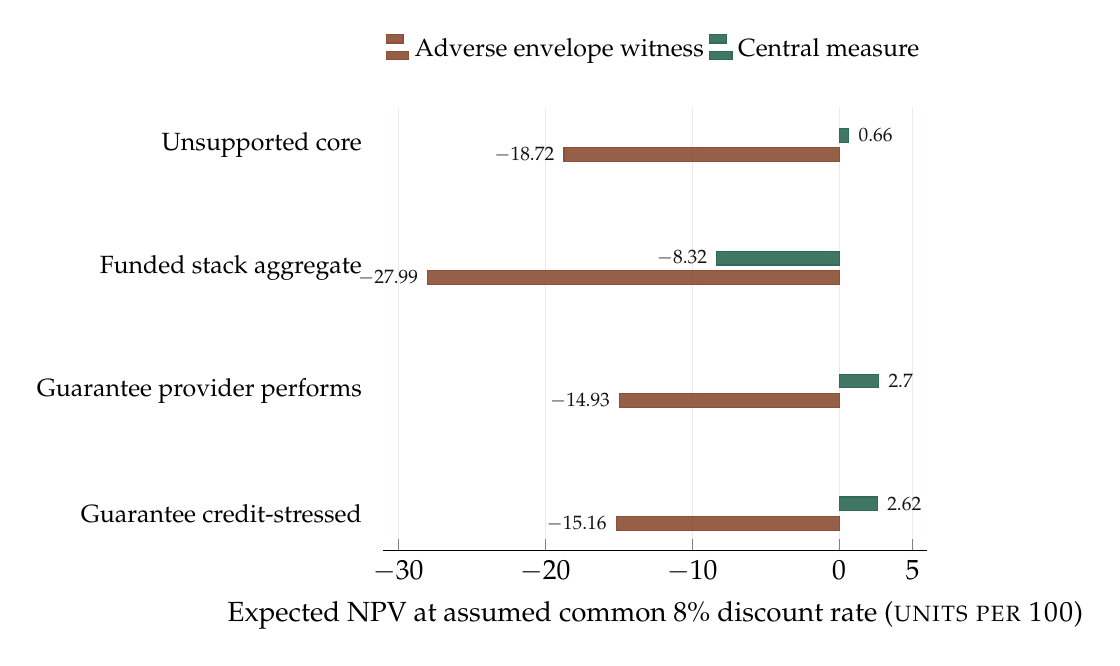
\begin{tikzpicture}
\begin{axis}[
  xbar,
  width=0.70\textwidth,
  height=72mm,
  xmin=-31,xmax=6,
  axis x line*=bottom,
  axis y line*=left,
  y axis line style={draw=none},
  ytick style={draw=none},
  symbolic y coords={Guarantee credit-stressed,Guarantee provider performs,Funded stack aggregate,Unsupported core},
  ytick=data,
  yticklabel style={font=\small,align=right},
  xtick={-30,-20,-10,0,5},
  xlabel={Expected NPV at assumed common 8\% discount rate (\demounit{})},
  xmajorgrids=true,
  grid style={draw=Mist},
  legend style={at={(0.5,1.08)},anchor=south,legend columns=2,draw=none,font=\small},
  bar width=5pt,
  nodes near coords={\pgfmathprintnumber[fixed,precision=2]{\pgfplotspointmeta}},
  nodes near coords style={font=\scriptsize},
  every axis plot/.append style={fill opacity=.92}
]
\addplot[fill=Rust,draw=Rust] coordinates {
  (-15.161094,Guarantee credit-stressed)
  (-14.925982,Guarantee provider performs)
  (-27.985093,Funded stack aggregate)
  (-18.717674,Unsupported core)};
\addplot[fill=Positive,draw=Positive] coordinates {
  (2.617773,Guarantee credit-stressed)
  (2.699617,Guarantee provider performs)
  (-8.321750,Funded stack aggregate)
  (0.661828,Unsupported core)};
\legend{Adverse envelope witness,Central measure}
\end{axis}
\end{tikzpicture}
\caption{Expected NPV comparison. The funded stack aggregate uses an assumed common 8\% discount rate; its individual classes have separate assumed rates. Guarantee values are before investor premium.}
\label{fig:npv}
\end{figure}

\begin{table}[htbp]
\centering
\caption{What each construction changes}
\label{tab:variants}
\small
\begin{tabularx}{\textwidth}{@{}P{0.25\textwidth}R R Y@{}}
\toprule
\textbf{Construction} & \textbf{Central NPV} & \textbf{Adverse NPV} & \textbf{Financial interpretation} \\
\midrule
Unsupported callable core & 0.66 & -18.72 & Milestone stops reduce unused draws; investor bears gross project loss and delay. \\
Funded stack, aggregate at 8\% & -8.32 & -27.99 & Principal-cash priority and horizon-shortfall subordination become explicit, but full prefunding adds drag and creates no project value. \\
30\% guarantee, provider performs & 2.70 & -14.93 & External provider cash reduces retained resolved loss; premium is excluded. \\
30\% guarantee, credit-stressed & 2.62 & -15.16 & Wrong-way provider default reduces promised delivery in adverse states. \\
\bottomrule
\end{tabularx}
\end{table}

\subsection{Funded first-loss and priority variant}

Investors subscribe 100 into the reserve at month zero and contribute 1 as a separate pool-cost call; project uses are funded from the reserve and are not counted again as investor contributions. Expected prefunding drag at the pool's assumed 8\% discount rate is 8.98 centrally. At their own assumed rates, the 0--20 first-loss class has central NPV \(-0.85\) at 15\%; the 20--100 priority class has central NPV \(-13.93\) at 8\%. Priority has negative NPV in every declared state. Aggregate stack NPV at the assumed common 8\% rate is \(-27.99/-8.32/6.72\) across adverse, central and favorable expected cases.

The result is not an argument against subordination. It shows that subordination must be funded and priced. Asset \(L_s\) and \(O_s\) remain unchanged, while tranche principal-cash shortfalls sum to \(Q_s\). The model does not attribute asset loss or outstanding principal causally to liability layers; rearranging the order of distributions cannot repair insufficient aggregate value.

\subsection{Partial-credit guarantee and provider capacity}

With full provider performance, central expected nominal guarantee payment is 2.99 at month 60, increasing investor receipts from 121.65 to 124.64. Gross resolved loss stays 9.98; investor-retained loss falls to 6.99; continuing exposure stays 8.52. The NPV improvement from 0.66 to 2.70 is the discounted value of an external transfer, not an improvement in projects.

The provider payment can reach 6.46 as an expected value over the probability envelope, while single-path payment can reach 27.00. The modeled all-in support gap is 28.47. Incorporating wrong-way provider credit raises the gap to 28.70 and reduces central/adverse investor NPV to 2.62/\(-15.16\). The guarantee therefore fails both sides of the proposed market: it does not make the investor robustly adequate, and the investor cannot fund the provider's declared requirement with a non-negative premium consistent with its own target.

\section{Investor value, risk and exposure}

\subsection{What could make the asset valuable}

The candidate can become attractive only through real economic changes, not labels. Five channels are legitimate:

\begin{enumerate}
  \item \textbf{Stronger assigned cash rights.} Enforceable commercial, licensing, royalty, capacity or offtake payments can increase expected and adverse cash without relying on company valuation.
  \item \textbf{Better milestone control.} Earlier, independently verified stopping rules can reduce expected draws and downside liquidity while preserving value-producing paths.
  \item \textbf{True diversification.} Projects using materially different technical routes, suppliers, jurisdictions and buyers can reduce common-tail concentration if the data support it.
  \item \textbf{A lower issue price or different participation.} Price and success-cash sharing can align expected NPV with the buyer's hurdle, subject to issuer viability and source budgets.
  \item \textbf{Explicit risk-bearing support.} A funded first-loss investor can take a defined issued-principal cash-shortfall layer \(Q\); a capable guarantor can cover a defined resolved asset-loss layer \(L\). Each transfers only the risk specified by its contract, and its cost, authority, liquidity and return requirement must be transparently financed.
\end{enumerate}

These channels can be compared because the standard holds accounting constant. If a proposed term improves NPV while receipts, price, timing and external transfers are unchanged, the improvement is suspect.

\subsection{Capital Mobilization Frontier v0.2: same-pool rejection and the conditional next channel}

Version 0.2 asks a narrower investor question than the construction comparison above: with the ten project paths, the box-and-simplex physical probability set in \cref{tab:states}, claim identifiers, lifetime market priority cap \(B=24\), assumed junior discount rate of 15\%, assumed investor discount rate of 8\% and zero junior target NPV held fixed, does any declared pair of success-cash participation \(q\) and funded junior issued principal \(A\) satisfy every element of the illustrative risk budget? The tested grids are

\[
q\in\{0.5,0.625,0.75,0.875,1\},\qquad
A\in\{10,20,30,40,50\},
\]

so the result covers exactly 25 candidates. It is enumeration, not interpolation or continuous optimization.

\begin{table}[htbp]
\centering
\caption{Complete finite-grid feasibility screen}
\label{tab:full-grid}
\small
\begin{tabular}{@{}lccccc@{}}
\toprule
\(q\backslash A\) & 10 & 20 & 30 & 40 & 50 \\
\midrule
0.500 & \(\times\) & \(\times\) & \(\times\) & \(\times\) & \(\times\) \\
0.625 & \(\times\) & \(\times\) & \(\times\) & \(\times\) & \(\times\) \\
0.750 & \(\times\) & \(\times\) & \(\times\) & \(\times\) & \(\times\) \\
0.875 & \(\times\) & \(\times\) & \(\times\) & \(\times\) & \(\times\) \\
1.000 & \(\times\) & \(\times\) & \(\times\) & \(\times\) & \(\times\) \\
\bottomrule
\end{tabular}
\tightnote{\(\times\) means that at least one declared return, tail-risk, incidence, WAL, first-loss or junior-concession constraint fails. The table reports every tested point; it says nothing about untested terms.}
\end{table}

The accounting layers must not be collapsed. The portfolio reports an aggregate project-outlay limit of 100 and an aggregate contractual asset-principal limit of 100. Their equality is a property of this retained at-par synthetic fixture, not an accounting identity. The v0.2 stack separately funds a reserve and total issued principal of \(K=100\); buyer-direct cost remains outside \(K\). In state \(s\), contractual writeoff \(L_s\) and continuing contractual principal \(O_s\) remain asset-ledger facts. Issued-principal cash shortfall is the liability fact

\[
Q_s=K-D_s,
\]

where \(D_s\) is principal cash distributable to the issued claims by the horizon. For a boundary \(A\), the junior claim covers \([0,A]\) in \(Q\)-shortfall coordinates and the market claim covers \([A,K]\), with market issued principal \(M=K-A\). Thus \(A\) allocates liability cash shortfall; it neither causes nor identifies asset loss.

The illustrative budget required non-negative robust market NPV margin; worst-case \(E[Q]/M\leq10\%\), Q-ES95/M \(\leq50\%\), Q-ES99/M \(\leq60\%\), and \(\Pr[Q>0]\leq35\%\); market negative-NPV probability \(\leq35\%\); NPV-shortfall ES95/M \(\leq60\%\) and ES99/M \(\leq70\%\); WAL \(\leq10\) years; \(A\leq50\); and junior NPV concession \(\leq50\). Aggregate NPV was deliberately left undeclared. These thresholds are invented research inputs, not observed institutional limits. A missing constraint does not silently bind.

\begin{table}[htbp]
\centering
\caption{Two disclosed points from the rejected 25-candidate v0.2 frontier}
\label{tab:v02frontier}
\small
\begin{tabularx}{\textwidth}{@{}P{0.12\textwidth}R R R R R@{}}
\toprule
\textbf{\((q,A;M)\)} & \textbf{Robust market NPV} & \textbf{Worst \(E[Q]/M\)} & \textbf{Q-ES95/99 over \(M\)} & \textbf{Max \(\Pr[Q>0]\)} & \textbf{Max \(\Pr[NPV<0]\)} \\
\midrule
\((1,20;80)\) & -25.73 & 27.38\% & 87.5\% / 87.5\% & 60\% & 100\% \\
\((1,50;50)\) & -5.57 & 12.16\% & 80\% / 80\% & 28\% & 54\% \\
\bottomrule
\end{tabularx}
\end{table}

No candidate passed every declared constraint; consequently the feasible set, nondominated feasible set and minimum tested feasible \(q\) are all empty. The larger junior layer at \((1,50)\) lowers market shortfall incidence, but still breaches the expected-\(Q\), both Q-tail and negative-NPV screens. This finding applies only to the declared finite grid, fixed terms, physical probability set and invented thresholds. It neither proves that an untested term fails nor establishes how an investor would price or buy the claim.

The next conditional channel is therefore not another relabelling of project loss. Holding the same \(q=1\), \(A=20\) claim and its future cash paths fixed, a priority-cap sensitivity selects \(B=24\), after which the issue-price/support module compares an investor's robust gross price ceiling \(P^*(h)\) with the issuer funding floor

\[
P_{\min}=\max(0,M+F-G),
\]

where \(F=0\) is issuer cost and \(G=20\) is an invented maximum non-repayable support sensitivity. With \(M=80\), the synthetic floor is 60. The supplied hurdle-sensitivity cases produce the following arithmetic windows:

The priority-cap record uses a \emph{separate, relaxed issue-price sensitivity budget}: expected \(Q/M\leq30\%\), Q-ES95/M and Q-ES99/M \(\leq90\%\), \(\Pr[Q>0]\leq60\%\), and WAL \(\leq5\) years. Those are not the strict frontier's 10\%, 50\%/60\%, 35\%, and ten-year limits. The strict 25-candidate frontier rejects this same \((q,A;M)=(1,20;80)\) point. A pass under the separate sensitivity limits is therefore not a frontier pass. Price and support can change NPV and the issue funding identity, but they cannot change \(Q\), Q-ES95/99, \(\Pr[Q>0]\), or WAL and cannot cure that fixed-risk failure.

\begin{table}[htbp]
\centering
\caption{Conditional same-pool issue-price/support windows}
\label{tab:pricewindows}
\scriptsize
\begin{tabularx}{\textwidth}{@{}R R R R Y@{}}
\toprule
\textbf{Assumed rate \(h\)} & \textbf{Robust ceiling \(P^*\)} & \textbf{Minimum support \(G_{\min}\)} & \textbf{Shortfall to \(G=20\)} & \textbf{Overlap with issuer floor 60} \\
\midrule
0\% & 74.58 & 5.42 & 0 & [60, 74.58] \\
5\% & 60.96 & 19.04 & 0 & [60, 60.96] \\
8\% & 54.27 & 25.73 & 5.73 & none \\
10\% & 50.31 & 29.69 & 9.69 & none \\
15\% & 41.90 & 38.10 & 18.10 & none \\
20\% & 35.17 & 44.83 & 24.83 & none \\
\bottomrule
\end{tabularx}
\end{table}

Here \(G_{\min}=\max(0,M+F-P^*)\) is the modeled no-rights support needed just to create overlap, and ``shortfall'' is \(\max(0,G_{\min}-20)\). These are conditional source-and-price identities, not market observations. The reference gross buyer price \(P_{\mathrm{ref}}=80\) exceeds every investor ceiling in the table. That reference, all six assumed rates and the support capacity are synthetic; settled support is zero; no support funding, escrow, authority, budget or settlement is evidenced; and no rate is empirically calibrated. Accordingly, the module finds arithmetic overlap only at 0\% and 5\%, finds none at the paper's assumed 8\% investor discount rate or higher, and finds no funded/escrowed-support-covered window at any assumed rate. The separate relaxed screen does not reverse the strict frontier rejection. The module does not estimate fair value, discover a discount curve, show investor demand, prove legal enforceability, authorize execution, establish financing additionality, or establish capital mobilization. A live next step requires independent buyer-price and hurdle evidence, verified issuer uses and costs, and a legally authorized, funded and settlement-ready support source.

\subsection{Exposure is multi-dimensional}

No single rating-like number is appropriate at the present stage. Investors should receive at least:

\begin{itemize}
  \item dated contribution and receipt distributions;
  \item expected NPV and probability of negative NPV at independently supported hurdles;
  \item resolved asset-loss tails for guarantee analysis, v0.2 issued-principal cash-shortfall expectation, incidence and ES95/ES99 for the funded stack, and NPV-shortfall VaR/ES at disclosed levels;
  \item continuing exposure, duration or weighted-average life where defined;
  \item project, stage, source, factor, buyer and provider concentrations;
  \item simultaneous-draw and peak cumulative liquidity requirements;
  \item adverse probability witnesses and factor attribution;
  \item provider expected payment, tail payment, collateral, unsecured exposure and wrong-way credit sensitivity; and
  \item separate mission additionality and impact evidence.
\end{itemize}

Expected return without these exposures is not an institutional description of the asset. Likewise, a low expected loss does not imply a tolerable tail, liquid price or small capital requirement.

\section{Empirical boundary and live-use conditions}

\subsection{Exact mechanics are conditional, not calibrated}

The engine is exact about the question it is given: it conserves dated cash and principal on each declared path and retains the probability witness that binds each robust result. It does not make the state space, cash paths, recoveries, probabilities or hurdle true. An expected loss computed from invented state weights is a synthetic sensitivity; a tail bound over analyst-declared probability limits is model ambiguity, not a sampling-confidence statement.

A mechanically senior tranche can therefore remain impossible to underwrite. More simulations, projects or attachment points cannot replace a complete, economically de-duplicated claim history with frozen inclusion rules, comparable terms and terminal or explicitly censored outcomes. Likewise, a modeled price ceiling cannot authenticate its own hurdle or establish market demand.

\subsection{Evidence needed to estimate rather than assume}

A future institutional study must independently admit three evidence objects:

\begin{enumerate}
  \item \textbf{Physical performance:} a frozen claim population containing resolved, unresolved, immature, disputed, denied and zero-loss cases; dated contributions, receipts, writeoffs and recoveries; visible exclusions; common-factor observations; missingness and censoring.
  \item \textbf{Market terms:} settled primary prices or executable quotes for sufficiently comparable rights, together with size, seniority, duration, liquidity, currency, costs and a hurdle that is not inferred from the target model.
  \item \textbf{Funding and support:} executed capital-call, warehouse or guarantee terms; provider identity, authority, capacity, collateral, concentration and actual settlement; no forecast refinancing counted as cash.
\end{enumerate}

The repository's controlled cohort binder preserves population and provenance, but it has no empirical authority until classification, comparability, exclusion timing and source truth are independently authenticated. The three public transaction dossiers improve mechanism design but do not identify a transferable loss distribution or discount-rate set; their precise limits are reported in \cref{app:transactions}. A calibrated model would additionally require a stated transfer method, effective sample size, estimation uncertainty, challenger specification and holdout or later-vintage validation.

\subsection{Decision boundary}

A live candidate should proceed only if a frozen data room and model release establish unique enforceable cash rights, effective milestone stops, reconciled funding, investor adequacy at evidenced price and hurdle, tolerable adverse exposure, capable support under joint stress, minimum and transparent concession, and incremental qualified capacity relative to a stated counterfactual. The economic arrangement may ultimately be classified as a loan, security, participation, fund interest, derivative, insurance contract or public contingent liability depending on facts and jurisdiction; this paper does not select that legal classification. The detailed contractual and diligence controls are retained in \cref{app:diligence}.

\section{Falsification conditions and limitations}

The investment thesis is falsified if any material condition below persists:

\begin{enumerate}
  \item Named cash rights are absent, unenforceable, overlapping or insufficient.
  \item Milestones cannot verifiably stop later draws.
  \item Material shared shocks are omitted or results depend on silent independence.
  \item Full contractual success participation still fails robust NPV.
  \item Simultaneous draws or continuing exposure create an unfunded liquidity need.
  \item Provider requirements exceed investor premium capacity.
  \item Guarantee authority, funding, collateral control or enforceability is absent.
  \item Market-hurdle evidence is circular, stale or incomparable.
  \item Transferability, legal perfection, limited recourse or insolvency remoteness fails.
  \item Concessionary support is hidden or is not demonstrably additional.
  \item The financing does not cause incremental qualified capacity or credible animal displacement.
\end{enumerate}

The current model is deliberately incomplete. It does not estimate live probabilities, fair value, liquidity discounts, tax, accounting classification, regulatory capital, endogenous behavior, strategic default, servicer failure, construction cost escalation, foreign exchange, commodity basis, dynamic refinancing, secondary-market price, moral hazard or investor demand. Joint states are finite and manually specified. Recovery is stylized. The 60-month horizon can classify economically valuable but unresolved claims as continuing exposure. Tail metrics are sensitive to state design and probability bounds. These limitations prevent the paper from supporting an issuance; they do not prevent it from defining what evidence an issuance would require.

\section{Implementation and reproducibility}

The analytical core is written in C++ and uses strict text configurations, deterministic scenario evaluation, exact cash-source and principal reconciliations, bounded-probability optimization, resolved asset-loss tails, issued-principal-cash-shortfall tails, NPV-shortfall tails, tranche waterfalls, guarantee payment, provider price decomposition and provider-credit stress. The maintained research repository includes model specifications, fixtures, command-line reporters, adversarial tests and verification records \citep{fca2026brief,fca2026term,fca2026analysis}.

For the paper's reported snapshot:

\begin{itemize}
  \item model date: 1 September 2026;
  \item exact portfolio: ten synthetic claims and nine complete joint states;
  \item monetary convention: synthetic \demounit{}, constant analysis-close basis;
  \item discounting: annual-effective, monthly exponents;
  \item reconciliation tolerance: \(10^{-9}\) for modeled floating identities;
  \item verification status: the tagged quantitative kernel is unchanged from the version 1.3 release, whose complete warnings-as-errors C++20 Emscripten 6.0.5 Release build and Node-driven suite passed 73 of 73 declared tests, including the strict five-file cohort loader, population-frame Evidence Gate, v0.2 asset-to-liability bridge, direct Claim Ledger integration, frontier core/parser/CLI regressions, issue-price browser target and published-WASM byte-parity check;
  \item immutable release identity: tag \texttt{fca-whitepaper-v2.0.0}; the tagged \href{https://github.com/savethebeesandseeds/naturalehia/blob/fca-whitepaper-v2.0.0/projects/fostering-cellular-agriculture/whitepaper/release-manifest-v2.0.tsv}{release manifest} records the paper-relevant source, fixture and released-PDF hashes;
  \item publication boundary: the proposed funding-liquidity extension in this paper has no released quantitative bridge output and is excluded from the tagged 73-test result;
  \item portable execution: the retained quantitative release evidence is produced by the pinned Emscripten container and Node, including every command-line report wrapper;
  \item paper toolchain: \texttt{latexmk} inside the Debian-based \texttt{documents-latex:bookworm} container.
\end{itemize}

The public browser interface is a readable analytical view of frozen synthetic results, and the same C++ kernel now has a strict WebAssembly build path. Browser interactivity does not itself prove parity or calibration: any published parity claim must remain tied to named structured-output fixtures, input hashes and retained cross-runtime tests.

\section{Open-standard and responsibility commitments}

Naturalehia retains no protocol fee, carried interest, instrument royalty or share of financed-company receipts for publishing or adopting this open standard. Underlying project claims may still assign capped commercial, licensing, royalty, capacity, offtake or exit cash to investors; without such rights there may be no investable asset. The zero-rent commitment reduces one conflict but does not improve cash flows or prove investment value.

The governing charter requires underwriting before advocacy, full visibility of risk transfer, transparent subsidy, no stronger claim than evidence, sponsor accountability, safety and food-integrity protection, conservative animal-impact attribution and an auditable go/no-go decision \citep{fca2026charter}. If rigorous analysis rejects a transaction, the mission is served by not spending scarce capital on terms that conceal failure.

\section{Conclusion}

The proposed Multi-Project Milestone Participation is a financial standard before it is a product. It defines a real candidate asset as a limited-recourse claim on dated, source-budgeted project cash and recoveries; represents unresolved exposure separately from loss; encodes shared shocks directly; and lets funded subordination allocate actual cash and horizon shortfall \(Q_s\), or guarantee support transfer defined asset loss, without confusing either operation with value creation.

The synthetic experiment gives the appropriate first conclusion. Pooling provides some ES95 benefit, but common risk dominates ES99. The central core NPV is slightly positive, yet the adverse permitted NPV is materially negative. Fully funded priority creates drag, and the guarantee adds useful external cash but still cannot satisfy both investor and provider constraints. The additive v0.2 frontier rejects every one of the 25 declared same-pool \((q,A)\) candidates. Its downstream issue-price/support sensitivity shows arithmetic overlap only under invented 0\% and 5\% discount-rate cases with uncommitted support, not at the assumed 8\% investor discount rate, and no overlap is funded or escrowed. None of the current constructions is shown financeable.

The next serious step is empirical: acquire enforceable project cash rights, milestone and recovery data, joint-risk evidence, investor price/hurdle observations and provider capacity terms in the common interface. A nonanticipative funding-liquidity layer can then test whether staged callable commitments or a warehouse reduce dead-cash drag without concealing provider, refinancing or settlement risk. Until that layer passes its accounting, eligibility, recovery and policy-timing controls, this paper claims no funding saving. With admissible facts and mechanics, the framework can test whether a revised instrument is valuable, what risks it distributes across projects and institutions, and how much explicit catalytic support is genuinely required.

\clearpage
\section*{Declarations}
\addcontentsline{toc}{section}{Declarations}

\textbf{Funding.} No external funding was received for this paper.\\
\textbf{Authorship and responsibility.} Naturalehia Research is the collective author. It is responsible for the research question, evidence boundary, model specification, calculations and release decision.\\
\textbf{Author economics.} Naturalehia retains no protocol fee, carried interest, instrument royalty or share of financed-company receipts from adoption of the published standard.\\
\textbf{Conflicts.} No ownership, employment, advisory, consulting or other financial relationship with a named issuer, investor, guarantor or project has been disclosed to or relied upon by this research; no named party is endorsed or admitted. This statement does not substitute for signed author and adviser disclosures before any live transaction or third-party publication.\\
\textbf{Computational assistance.} AI-assisted drafting and code review were used. All claims, model boundaries, source selection, code, tests and release decisions remain the author's responsibility.\\
\textbf{External review.} This working paper has not been externally peer reviewed.\\
\textbf{Data and code.} Source, configurations, documentation and tests for this paper are fixed by release tag \href{https://github.com/savethebeesandseeds/naturalehia/tree/fca-whitepaper-v2.0.0/projects/fostering-cellular-agriculture}{\texttt{fca-whitepaper-v2.0.0}}. The numerical case is synthetic.\\
\textbf{Use boundary.} The paper is research, not professional advice or an offer. Independent qualified review is required before any transaction.

\bibliographystyle{plainnat}
\begingroup
\small
\bibliography{references}
\endgroup

\clearpage
\appendix

\section{Economic identities and proofs}
\label{app:proofs}

\textbf{Proof of Proposition 1.}
Fix a state \(s\) and month \(t\). An exhaustive waterfall partitions the cash available to issued claims, so that
\[
\sum_j CF_{j,s}(t)=CF^{\mathrm{pool}}_s(t),
\]
with no cash assigned twice and no residual omitted. Present value at a common annual-effective hurdle \(h\) is a linear operator:
\[
\sum_j\sum_t\frac{CF_{j,s}(t)}{(1+h)^{t/12}}
=\sum_t\frac{CF^{\mathrm{pool}}_s(t)}{(1+h)^{t/12}}.
\]
Thus tranche cash and tranche NPV aggregate to the pool amounts in every state. Different tranche hurdles can change quoted investment values, but they do not change pool cash. \(\square\)

\textbf{Proof of Proposition 2.}
For a guarantee with delivered external payment \(G_s(t)\), investor cash is
\[
CF^{\mathrm{protected}}_s(t)=CF^{\mathrm{unprotected}}_s(t)+G_s(t).
\]
Project receipts, gross project loss and continuing principal are unchanged because \(G_s(t)\) originates outside the reference assets. Before any premium or provider fee,
\[
V^{\mathrm{protected}}_s(h)-V^{\mathrm{unprotected}}_s(h)
=\sum_t\frac{G_s(t)}{(1+h)^{t/12}}.
\]
The identity concerns cash actually delivered; a promise, limit or expected payment is not cash. \(\square\)

\textbf{Proof of Proposition 3.}
Expected shortfall under one fixed physical measure \(p\) is coherent and therefore subadditive \citep{artzner1999coherent,rockafellar2000cvar}:
\[
\operatorname{ES}^{p}_{\alpha}\!\left(\sum_i\ell_i\right)
\leq\sum_i\operatorname{ES}^{p}_{\alpha}(\ell_i).
\]
Rearrangement gives \(D_\alpha^p\geq0\). Equality can hold when the same common state occupies the relevant tail for every claim and their sum. This proof does not permit subtraction of endpoints optimized under different probability witnesses; any robust comparison must retain a common measure or solve the combined objective directly. \(\square\)

\section{Notation}

\begin{longtable}{@{}P{0.18\textwidth}P{0.73\textwidth}@{}}
\caption{Principal notation}\label{tab:notation}\\
\toprule
\textbf{Symbol} & \textbf{Definition} \\
\midrule
\endfirsthead
\toprule
\textbf{Symbol} & \textbf{Definition} \\
\midrule
\endhead
\(i,s,t\) & Project, complete joint state and month. \\
\(d_{ist}\) & Project draw funded by investors. \\
\(b_{ist}\) & Contractual-principal balance. \\
\(r^P_{ist}\) & Contractual-principal cash returned. \\
\(x_{ist}\) & Assigned non-principal success cash. \\
\(\rho_{ist}\) & Recovery cash. \\
\(\ell_{is}\) & Resolved contractual-principal loss. \\
\(u_{is}\) & Continuing contractual principal at horizon. \\
\(e_{is}\) & Evidenced conversion or other non-cash extinguishment. \\
\(L_s\) & Aggregate resolved contractual-principal writeoff, \(\sum_i\ell_{is}\). \\
\(O_s\) & Aggregate continuing contractual principal, \(\sum_i u_{is}\). \\
\(A_{is}\) & Acquisition and primary-funding reserve use for project \(i\) in state \(s\), excluding buyer direct cost. \\
\(R_i\) & Project reserve limit, \(\max_s A_{is}\). \\
\(R\) & Aggregate reserve subscription and issued principal, \(\sum_iR_i\). \\
\(A_s\) & Aggregate state acquisition and primary-funding use, \(\sum_iA_{is}\). \\
\(U_s\) & Unused reserve returned at horizon, \(R-A_s\). \\
\(P_s\) & Contractual-principal cash received by the analysis horizon. \\
\(D_s\) & Principal cash distributable to issued claims, \(\min(R,P_s+U_s)\). \\
\(Q_s\) & Horizon issued-principal cash shortfall, \(R-D_s\); not an accounting impairment or recovery estimate. \\
\(S_s\) & Cash above unpaid issued principal, \(\max(0,P_s+U_s-R)\). \\
\(a_j,d_j\) & Attachment and detachment of tranche \(j\) in \(Q_s\)-shortfall coordinates. \\
\(K\) & Funded reserve and top issued-principal stack detachment in the v0.2 frontier; equal to \(R\) for its supplied stack template. \\
\(A\) & Funded junior issued-principal boundary in \(Q\)-shortfall coordinates; not causal attribution of asset loss. \\
\(M\) & Market issued principal, \(K-A\), excluding additional buyer-direct and pool-cost calls. \\
\(CF_s(t)\) & Investor net cash at month \(t\) in state \(s\). \\
\(V_s(h)\) & State NPV at annual-effective investor hurdle \(h\). \\
\(p\in\mathcal P\) & Admissible physical probability measure. \\
\(q\) & Participation share in assigned success cash. \\
\(B\) & Priority lifetime non-principal cash cap. \\
\(g\) & Guarantee share of final resolved loss. \\
\(\Gamma\) & Guarantee provider's legal cash cap. \\
\(G_s\) & Provider payment in state \(s\). \\
\(P_0\) & Issue price or investor premium, when applicable. \\
\(D_\alpha\) & Pooling diversification benefit at tail level \(\alpha\). \\
\bottomrule
\end{longtable}

\section{Complete synthetic claim schedule}

\begin{longtable}{@{}rP{0.29\textwidth}P{0.12\textwidth}rP{0.17\textwidth}P{0.16\textwidth}@{}}
\caption{Ten synthetic claims}\label{tab:claims}\\
\toprule
\# & \textbf{Claim} & \textbf{Stage} & \textbf{Limit} & \textbf{Draws m0/12/24} & \textbf{Performing receipt} \\
\midrule
\endfirsthead
\toprule
\# & \textbf{Claim} & \textbf{Stage} & \textbf{Limit} & \textbf{Draws m0/12/24} & \textbf{Performing receipt} \\
\midrule
\endhead
1 & Cell-line and media platform & Research & 6 & 2.4 / 1.8 / 1.8 & 11.40 at m60 \\
2 & Serum-free media platform & Research & 7 & 2.8 / 2.1 / 2.1 & 12.95 at m60 \\
3 & Cultivated beef pilot & Pilot & 8 & 2.8 / 2.8 / 2.4 & 14.00 at m54 \\
4 & Cultivated poultry pilot & Pilot & 9 & 3.15 / 3.15 / 2.7 & 15.75 at m54 \\
5 & Continuous-perfusion demonstration & Demo & 10 & 3.0 / 3.0 / 4.0 & 16.50 at m48 \\
6 & Food-grade scaffold pilot & Pilot & 7 & 2.45 / 2.45 / 2.1 & 11.90 at m54 \\
7 & First-industrial beef facility & First industrial & 15 & 3.75 / 5.25 / 6.0 & 23.25 at m48 \\
8 & First-industrial poultry facility & First industrial & 14 & 3.5 / 4.9 / 5.6 & 21.70 at m48 \\
9 & Cultivated-fat demonstration & Demo & 8 & 2.4 / 2.4 / 3.2 & 13.20 at m48 \\
10 & Repeat modular production line & Repeat & 16 & 3.2 / 4.8 / 8.0 & 24.00 at m42 \\
\midrule
 & \textbf{Total} & & \textbf{100} & & \textbf{164.65} \\
\bottomrule
\end{longtable}

\section{Accounting and waterfall controls}

Every evaluated state is subject to the following controls before reporting:

\begin{enumerate}
  \item in the callable core, investor contributions equal project outlays plus explicit pool costs and any separately stated premium;
  \item in the funded stack, investor contributions equal reserve subscription plus separate buyer-direct-cost and pool-cost calls; project acquisition and primary-funding uses consume reserve and are not counted again;
  \item project receipts equal commercial plus licensing/royalty plus recovery plus other named project-source cash;
  \item provider payments are external and never included in project-source cash;
  \item principal returned, extinguished, continuing and lost equals opening plus created principal;
  \item asset \(L_s\) and \(O_s\) are preserved separately, issued principal satisfies \(R=D_s+Q_s\), and tranche principal-cash shortfalls sum to \(Q_s\);
  \item tranche distributions do not exceed cash available under the waterfall;
  \item guarantee retained loss plus delivered provider payment equals gross resolved loss when full coverage terms apply, subject to the cap;
  \item probability weights remain non-negative, within bounds and sum to one; and
  \item each robust endpoint retains its optimizing probability witness.
\end{enumerate}

The consolidated model reports zero residual for the declared source, principal, tranche and protection reconciliations in the ten-claim fixture. A zero accounting residual proves internal conservation only; it does not validate an economic input.

\section{Controlled public transaction records}
\label{app:transactions}

\begin{table}[htbp]
\centering
\caption{Public-financing dossiers used for mechanism research, not calibration}
\label{tab:transaction-evidence}
\small
\begin{tabularx}{\textwidth}{@{}P{0.19\textwidth}P{0.31\textwidth}Y@{}}
\toprule
\textbf{Record} & \textbf{Publicly supported mechanism} & \textbf{Why it cannot identify price or loss} \\
\midrule
Liberation Labs, 2024--2025 \citep{fca2026liberationdossier} & Private secured notes with promised interest and a conversion feature for a fermentation facility. & Issuance clustering, all-in buyer cash, conversion, security, priority, recovery and expected-cash reconstruction remain incomplete. \\
Solar Foods Factory 01, 2022--2025 \citep{fca2026solarfoodsdossier} & Amortizing bank facility for a gas-fermentation protein facility, with capitalized commission, floating-rate terms, named export-credit guarantors and audited aggregate repayments. & The complete lender price, claim-level settlement, guarantee cash, default recovery and comparable adjustment bridge remain unavailable; gas-fermentation protein is not the same operating-risk class as cultivated-meat tissue production. \\
Meatable Innovation Credit, 2024 \citep{fca2026meatabledossier,agronomics2025meatabledissolution} & Issuer-reported public-credit award directed to cultivated-meat productivity and cost reduction; a later investor announcement reports a resolution to dissolve and wind down the operating group after continued funding was unavailable. & The adverse company and equity-investor outcome does not identify credit default, outstanding principal, acceleration, remission, priority, recovery or settlement; generic programme terms are not award-specific cash. \\
\bottomrule
\end{tabularx}
\end{table}
\FloatBarrier

None of these records enters the hurdle-evidence engine or calibrates the ten-claim pool. A controlled dossier preserves the source boundary; it does not mean that every cited web source was successfully byte-retained, and each source manifest reports retention status explicitly.

\section{Live-issuance diligence checklist}
\label{app:diligence}

\begin{longtable}{@{}P{0.22\textwidth}P{0.47\textwidth}P{0.22\textwidth}@{}}
\caption{Institutional work required beyond the research model}\label{tab:diligence}\\
\toprule
\textbf{Domain} & \textbf{Required evidence or decision} & \textbf{Failure consequence} \\
\midrule
\endfirsthead
\toprule
\textbf{Domain} & \textbf{Required evidence or decision} & \textbf{Failure consequence} \\
\midrule
\endhead
Reference assets & Executed claim schedule, unique rights, eligibility, substitution, transfer and servicing & Asset pool is undefined or double counted \\
Technical milestones & Objective predicates, verifier authority, cure, dispute and stop-draw mechanics & Milestone control has no economic force \\
Cash sources & Named payer, amount, date, source budget, priority and enforceability & Expected return is not an owned cash right \\
Dependence & Common-factor taxonomy, project mappings, joint observations and expert challenge & Pooling benefit is overstated \\
Recovery & Security, collateral, asset control, costs, timing and historical support & Loss is understated \\
Investor market & Comparable expected cash, issue price, constraints and evidenced hurdle & Adequacy test is circular \\
Protection provider & Authority, appropriation/funding, cap, collateral, claims and credit & Support may fail when needed \\
Legal structure & Classification, perfection, bankruptcy remoteness, limited recourse and tax & Waterfall or transfer may be unenforceable \\
Public purpose & Additionality, minimum concessionality, beneficiary, monitoring and clawback & Subsidy is hidden or unjustified \\
Animal impact & Qualified output, substitution baseline, attribution and assurance & Welfare claim is not permitted \\
\bottomrule
\end{longtable}

\vspace{-\baselineskip}
\enlargethispage{\baselineskip}
\section{Interpretive boundary}

This white paper is the concise technical synthesis of a larger open research program. Detailed format specifications, test fixtures, verification reports and candidate transaction dossiers remain in the repository. They are intentionally not reproduced here. The paper controls the public financial argument; the machine-readable sources control the implemented mechanics. If the two conflict, the stricter evidence boundary and the reproducible source calculations govern until the paper is corrected.

\end{document}
